\documentclass[professionalfont]{beamer}

\usepackage{graphicx}
\usepackage{newtxtext,newtxmath}
\usepackage[backend=bibtex]{biblatex} 
\addbibresource{ref.bib}
\renewcommand*{\bibfont}{\scriptsize}

\usetheme{default}
\usecolortheme{seagull}

\setbeamertemplate{navigation symbols}{}
\setbeamertemplate{itemize item}{\textbullet} 
\setbeamertemplate{bibliography item}[text]
\setbeamertemplate{title page}{
    \begin{center}
        {\textcolor{blue}{\textbf{\fontsize{13}{14}\selectfont
        Chain-of-Thought Prompting Elicits Reasoning \\
        in Large Language Models}}} \\[1.5cm]
        
        {\fontsize{9}{14}\selectfont Jason Wei, et al \\[0.3cm]
        Google Research, Brain Team \\[0.3cm]
        NeurIPS 2022}
    \end{center}
}
% ------------------ Title ------------------

\begin{document}
\frame{\titlepage}

\begin{frame}
\begin{center}
    { \textbf{\textcolor{blue}{ {\fontsize{12}{14}\selectfont Abstract} }} }
\end{center}
\\[0.5cm]

{\fontsize{10}{14}\selectfont 
\begin{itemize}
    \item \textit{Chain-of-Thought Prompting}
    
    - Reasoning ability emerges naturally in large models

    \\[0.2cm]
    
    \item Reasoning Experiments

    - Arithmetic / Commonsense / Symbolic

    - GPT-3, LaMDA, PaLM, etc.

    - For each model, variate parameter size

    - Compare standard prompting, CoT, and supervised SOTA

    \\[0.2cm]

    \item Results

    - As model becomes larger, CoT outperforms SOTA

    - Limitations: Mimicking, Manual exemplar cost
\end{itemize}
}

\end{frame}
% ------------------ Contents ------------------

\begin{frame}
\begin{center}
    { \textbf{\textcolor{blue}{ {\fontsize{12}{14}\selectfont Abstract} }} }
\end{center}
\\[0.2cm]

\begin{center}
    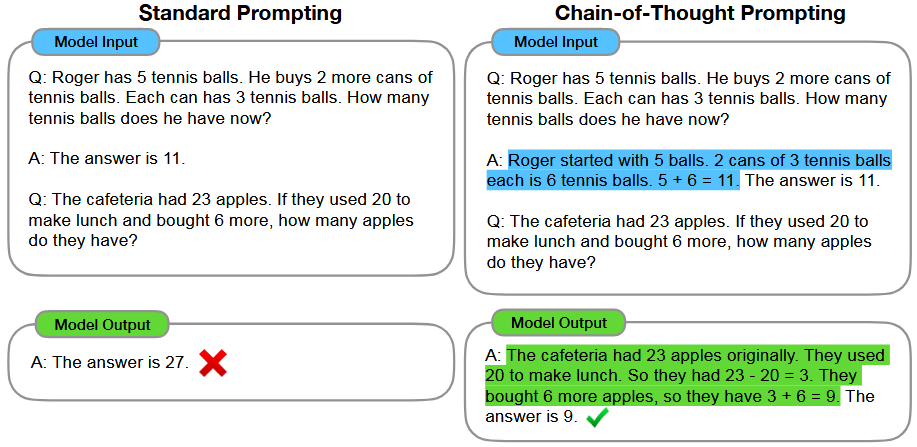
\includegraphics[width=1.0\textwidth]{figure1.png}
\end{center}


{\fontsize{10}{14}\selectfont 
- Reasoning abilities emerge naturally via Chain-of-Thought (CoT)
    
- Experiments on arithmetic, commonsense, and symbolic reasoning tasks
}

\end{frame}
% ------------------ Slide 1 ------------------

\begin{frame}
\begin{refsection}

\begin{center}
    { \textbf{\textcolor{blue}{ {\fontsize{12}{14}\selectfont Introduction} }} }
\end{center}
\\[0.5cm]

{\fontsize{10}{14}\selectfont 
\begin{itemize}
    \item Few-shot prompting \cite{gpt3}
    
    - We could perform unsupervised learning
    
    - However, it was poor at `Reasoning'

    \\[0.3cm]

    \item \textit{Chain-of-thought}

    - [Input, Chain of thought, Output] is given

    - Decomposes problem into subproblems

    - Provides interpretable window for debugging

    - Potentially applicable for any tasks
\end{itemize}
}

\vspace{0.3cm}
\hrule
\printbibliography

\end{refsection}
\end{frame}
% ------------------ Slide 2 ------------------

\begin{frame}
\begin{center}
    { \textbf{\textcolor{blue}{ {\fontsize{12}{14}\selectfont Arithmetic Reasoning - Result} }} }
\end{center}

\begin{columns}
\column{0.5\textwidth}
    {\fontsize{10}{14}\selectfont 
    \begin{itemize}
        \item Benchmarks

        - GSM8K \\
        - SVAMP \\
        - ASDiv \\
        - AQuA \\
        - MAWPS \\

        \\[0.3cm]

        \item CoT is efficient when

        - model is larger

        - problems are complicated
    \end{itemize}
    }
\column{0.5\textwidth}
    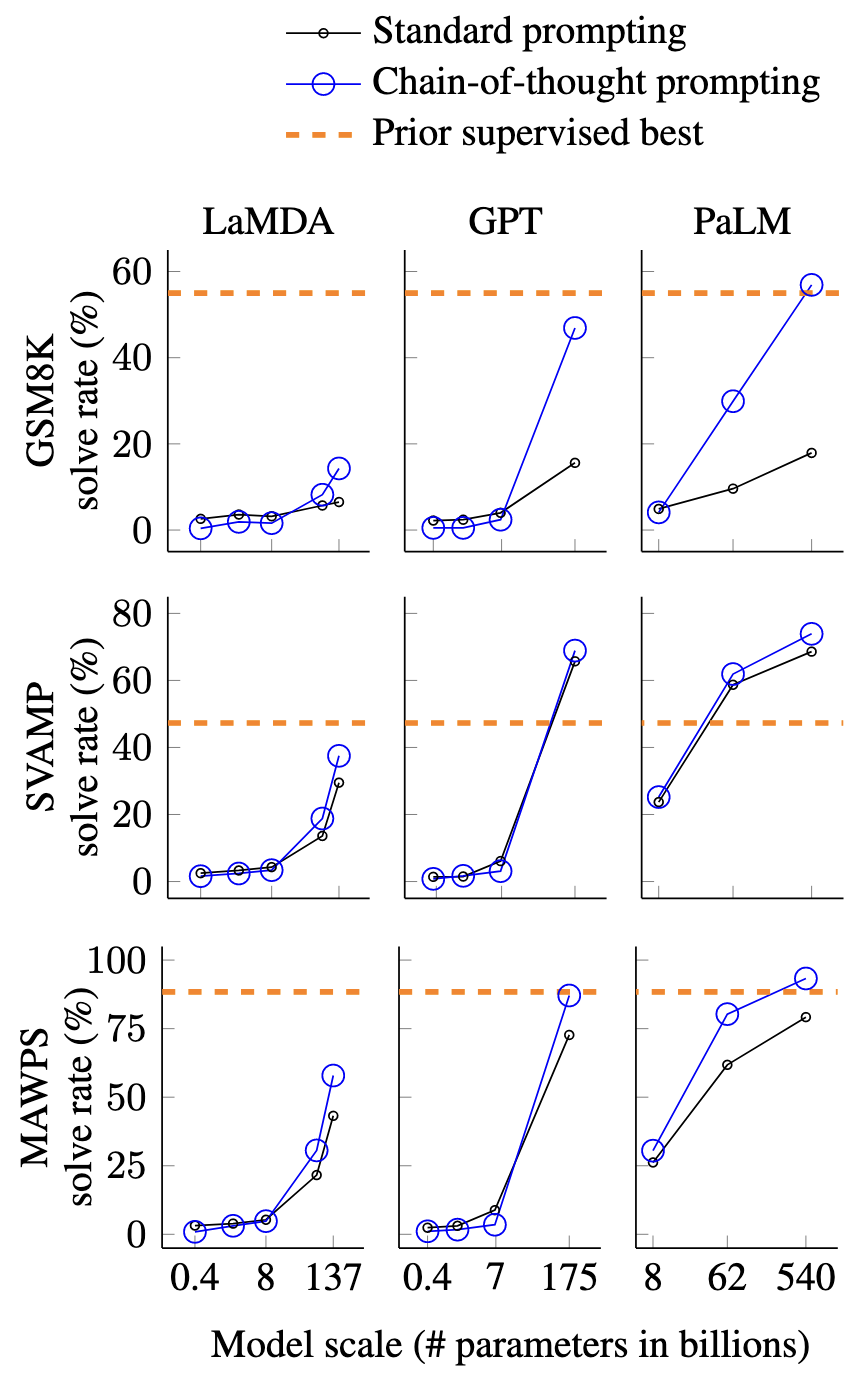
\includegraphics[width=0.9\linewidth]{figure4.png}
\end{columns}

\end{frame}
% ------------------ Slide 3 ------------------

\begin{frame}
\begin{center}
    { \textbf{\textcolor{blue}{ {\fontsize{12}{14}\selectfont Arithmetic Reasoning - Ablation} }} }
\end{center}
\\[0.3cm]

\begin{columns}
\column{0.5\textwidth}
    {\fontsize{10}{14}\selectfont 
    \begin{itemize}
        \item Equation only

        - Only helpful for short problems

        \\[0.3cm]

        \item Variable compute only

        - Length of CoT is given

        - No improvement

        \\[0.3cm]

        \item Reasoning after answer

        - No improvement
    \end{itemize}
    }
\column{0.5\textwidth}
    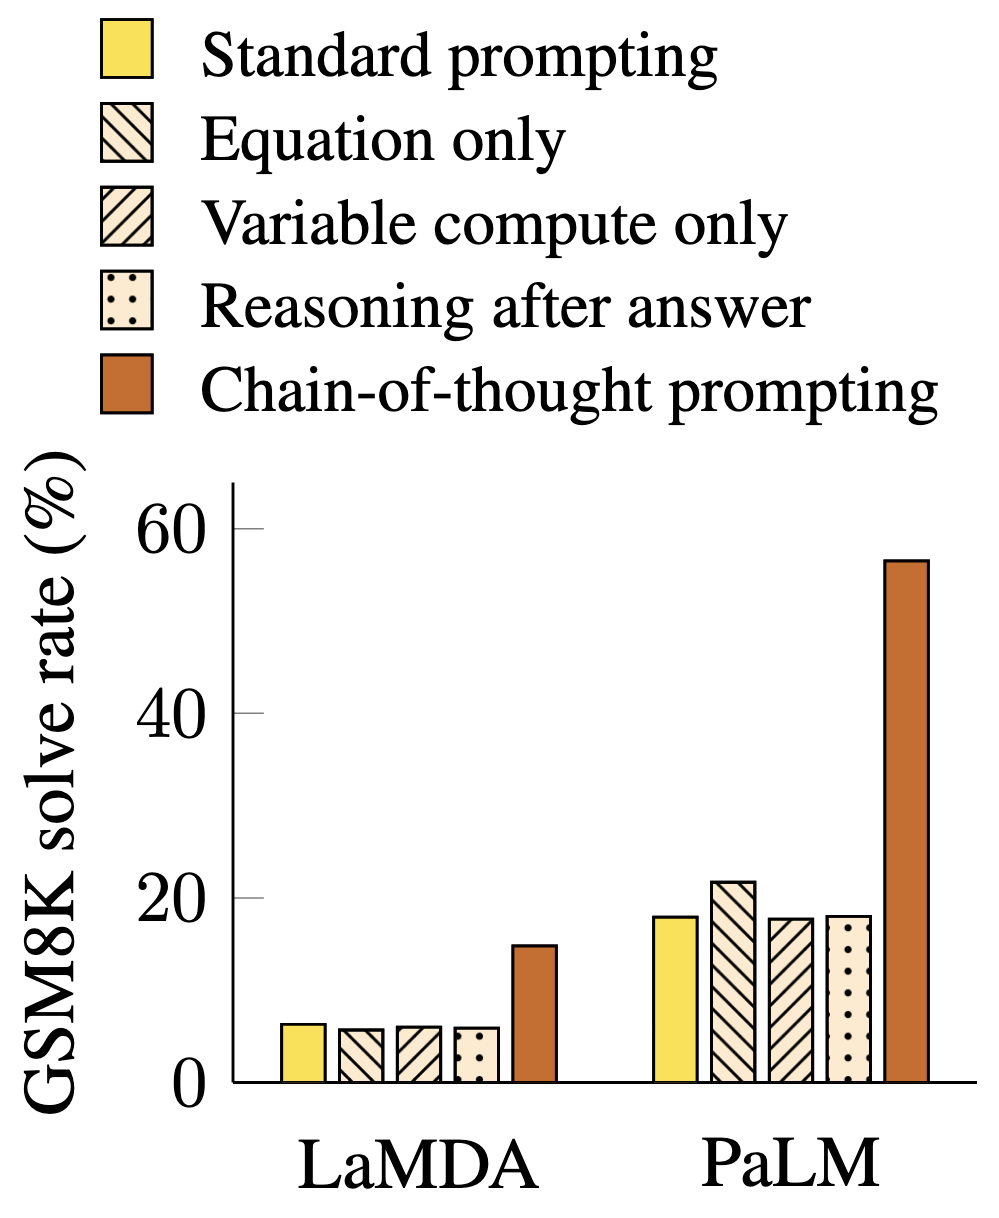
\includegraphics[width=0.9\linewidth]{figure5.png}
\end{columns}

\end{frame}
% ------------------ Slide 4 ------------------

\begin{frame}
\begin{center}
    { \textbf{\textcolor{blue}{ {\fontsize{12}{14}\selectfont Arithmetic Reasoning - Robustness} }} }
\end{center}
\\[0.3cm]

\begin{columns}
\column{0.5\textwidth}
    {\fontsize{10}{14}\selectfont 
    \begin{itemize}
        \item Sensitivity to exemplars

        - Different exemplar annotators

        - GSM8K Training exemplars

        \\[0.7cm]

        \item Result

        - All CoT outperformed standard

        - CoT is robust to linguistic style
    \end{itemize}
    }
\column{0.5\textwidth}
    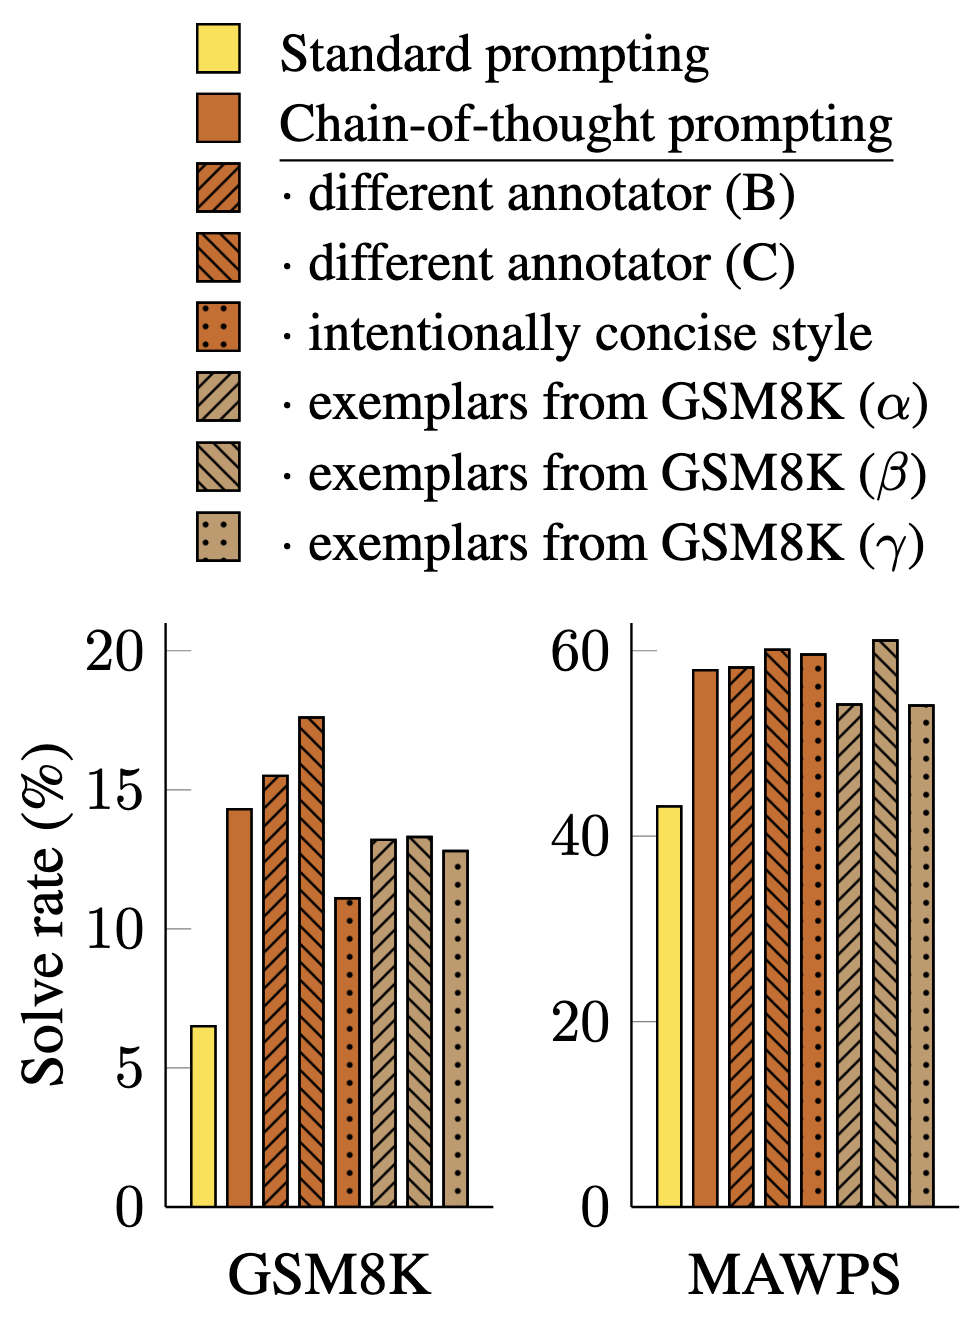
\includegraphics[width=0.9\linewidth]{figure6.png}
\end{columns}

\end{frame}
% ------------------ Slide 5 ------------------

\begin{frame}
\begin{center}
    { \textbf{\textcolor{blue}{ {\fontsize{12}{14}\selectfont Commonsense Reasoning} }} }
\end{center}
\\[0.3cm]

\begin{center}
    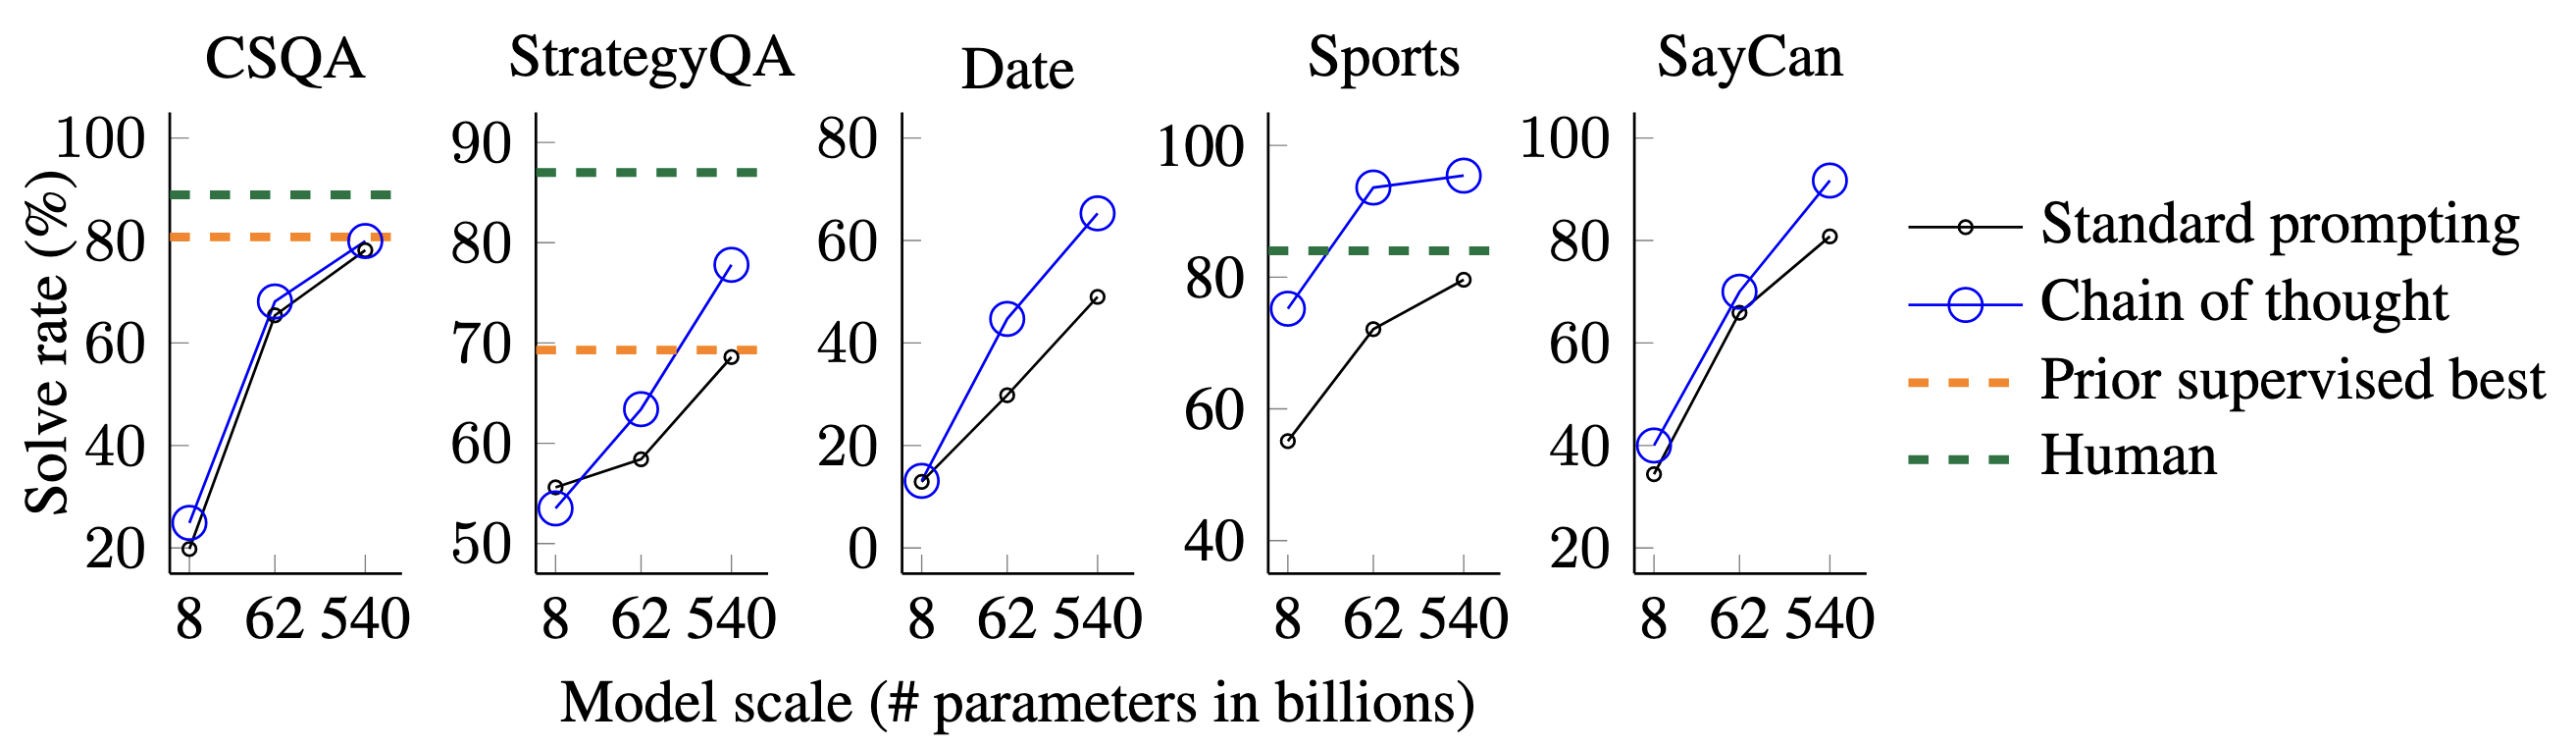
\includegraphics[width=1.0\textwidth]{figure7.png}
\end{center}

{\fontsize{10}{14}\selectfont 
\begin{itemize}
    \item Benchmarks
    
    - CSQA, StrategyQA, Date, Sports, SayCan

    \\[0.2cm]

    \item Experimental setup

    - Same as prior section
\end{itemize}
}

\end{frame}
% ------------------ Slide 6 ------------------

\begin{frame}
\begin{center}
    { \textbf{\textcolor{blue}{ {\fontsize{12}{14}\selectfont Symbolic Reasoning} }} }
\end{center}
\\[0.2cm]

\begin{columns}
\column{0.5\textwidth}
    {\fontsize{10}{14}\selectfont 
    \begin{itemize}
        \item Last letter concatenation

        - ``Amy Brown" \( \rightarrow \) yn

        - Challenging than first letter

        \\[0.3cm]

        \item Coin flip

        - People flip or don’t flip the coin

        - Asks the model to answer whether a coin is still heads up

        \\[0.3cm]

        \item Results

        - Performed well even in OOD

        - Length generalization by CoT
    \end{itemize}
    }
\column{0.5\textwidth}
    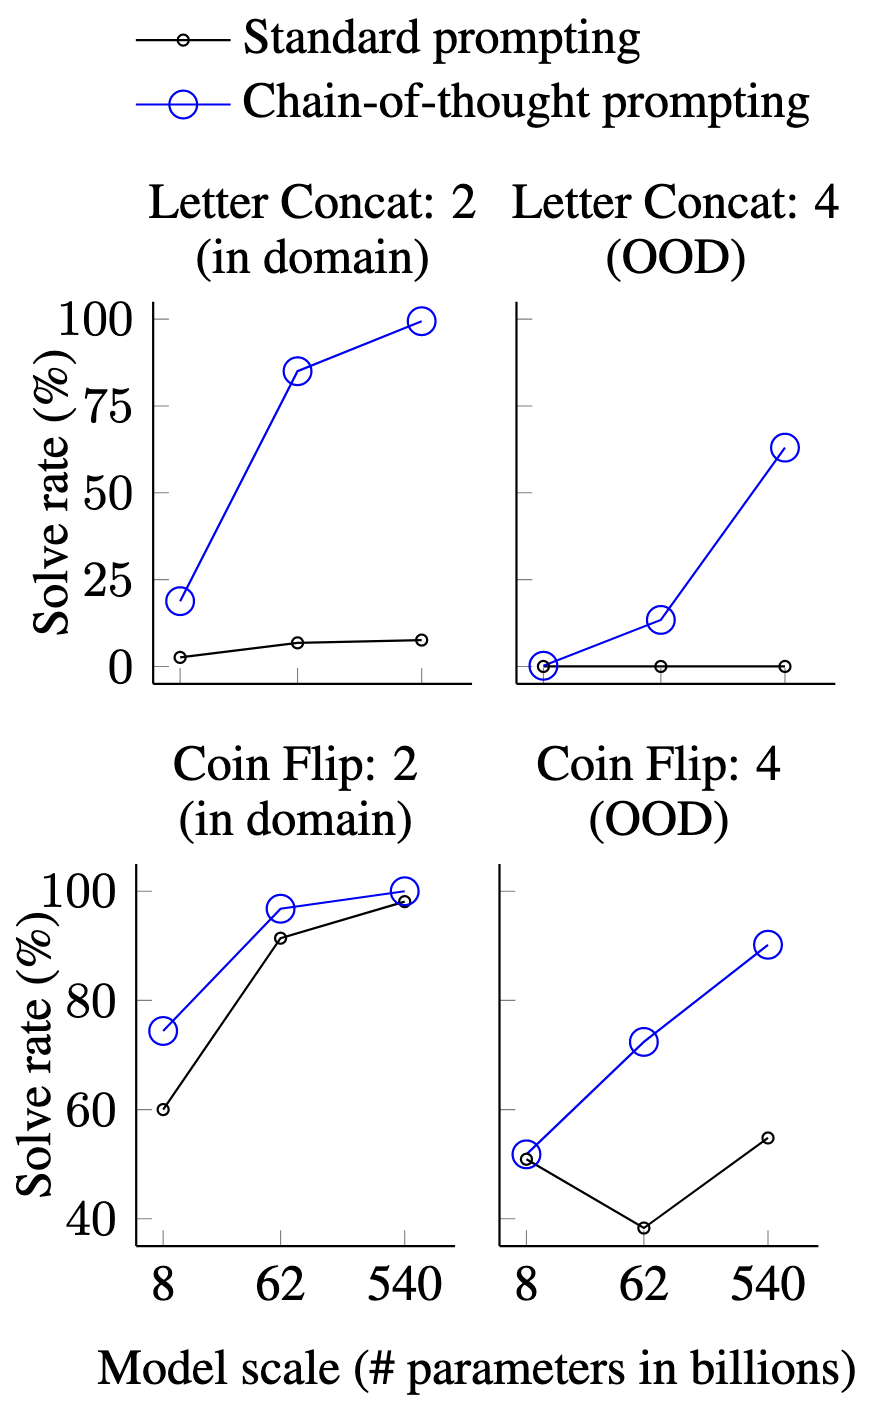
\includegraphics[width=0.9\linewidth]{figure8.png}
\end{columns}

\end{frame}
% ------------------ Slide 7 ------------------

\begin{frame}
\begin{center}
    { \textbf{\textcolor{blue}{ {\fontsize{12}{14}\selectfont Conclusion} }} }
\end{center}
\\[0.5cm]

{\fontsize{10}{14}\selectfont 
\begin{itemize}
    \item Chain-of-Thought performance
    
    - Standard prompting has a flat scaling curve

    - CoT has dramatically increasing scaling curves

    \\[0.2cm]

    \item It raises more questions

    - How much improvement with a further increase in model scale?

    - What other prompting methods would be there?

    \\[0.2cm]

    \item Limitation

    - Open question: Is it actually ``Reasoning"?

    - Cost of manually augmenting exemplars

    - There is no guarantee of correct reasoning paths

    - CoT appears only at large models
\end{itemize}
}
\end{frame}
% ------------------ Slide 6 ------------------

\end{document}
